\documentclass[tikz,border=8pt]{standalone}
\usepackage[utf8]{inputenc}\usetikzlibrary{positioning,fit,arrows.meta,shapes.geometric}
\definecolor{navy}{HTML}{17365D}\definecolor{teal}{HTML}{1F7A8C}\definecolor{soft}{HTML}{EAF4F6}
\tikzset{actor/.style={draw=navy,rounded corners,fill=white,minimum width=3.1cm,minimum height=.72cm,font=\bfseries\small},usecase/.style={draw=teal,ellipse,fill=soft,minimum width=6.1cm,minimum height=.72cm,align=center,font=\small},link/.style={draw=navy,-{Latex[length=2mm]},thin}}
\begin{document}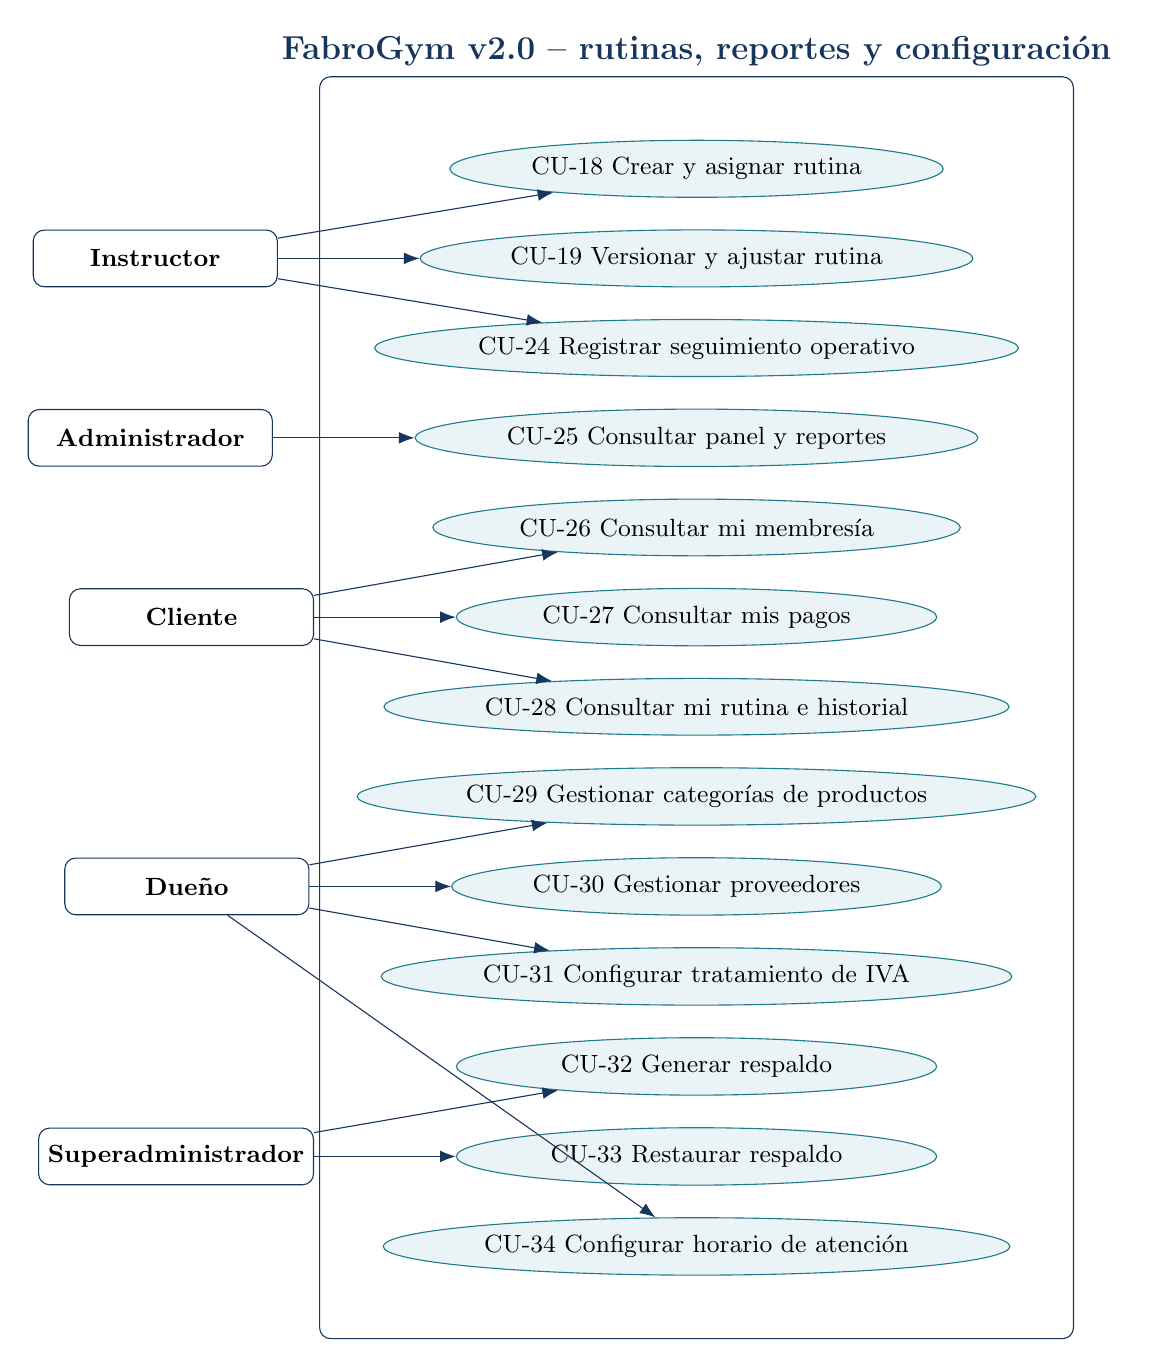
\begin{tikzpicture}[node distance=4mm and 15mm]
\node[usecase] (c18) {CU-18 Crear y asignar rutina};
\node[usecase,below=of c18] (c19) {CU-19 Versionar y ajustar rutina};
\node[usecase,below=of c19] (c24) {CU-24 Registrar seguimiento operativo};
\node[usecase,below=of c24] (c25) {CU-25 Consultar panel y reportes};
\node[usecase,below=of c25] (c26) {CU-26 Consultar mi membresía};
\node[usecase,below=of c26] (c27) {CU-27 Consultar mis pagos};
\node[usecase,below=of c27] (c28) {CU-28 Consultar mi rutina e historial};
\node[usecase,below=of c28] (c29) {CU-29 Gestionar categorías de productos};
\node[usecase,below=of c29] (c30) {CU-30 Gestionar proveedores};
\node[usecase,below=of c30] (c31) {CU-31 Configurar tratamiento de IVA};
\node[usecase,below=of c31] (c32) {CU-32 Generar respaldo};
\node[usecase,below=of c32] (c33) {CU-33 Restaurar respaldo};
\node[usecase,below=of c33] (c34) {CU-34 Configurar horario de atención};
\node[draw=navy,rounded corners,fit=(c18)(c34),inner sep=8mm,label={[font=\bfseries\large,text=navy]above:FabroGym v2.0 -- rutinas, reportes y configuración}] {};
\node[actor,left=18mm of c19] (ins) {Instructor};
\node[actor,left=18mm of c25] (ad) {Administrador};
\node[actor,left=18mm of c27] (cl) {Cliente};
\node[actor,left=18mm of c30] (du) {Dueño};
\node[actor,left=18mm of c33] (sa) {Superadministrador};
\foreach \x in {c18,c19,c24}\draw[link] (ins)--(\x);
\draw[link] (ad)--(c25);
\foreach \x in {c26,c27,c28}\draw[link] (cl)--(\x);
\foreach \x in {c29,c30,c31,c34}\draw[link] (du)--(\x);
\foreach \x in {c32,c33}\draw[link] (sa)--(\x);
\end{tikzpicture}\end{document}
